
A Pass in LLVM is the basic unit that is required to perform certain actions against LLVM IR. It is similar to a single production step in a factory, where the products that need to be processed are LLVM IR and the factory workers are the Passes. In the same way that a normal factory usually has multiple manufacturing steps, LLVM also consists of multiple Passes that are executed in sequential order, called the Pass pipeline. Figure 9.1 shows an example of the Pass pipeline:

\hspace*{\fill} \\ %插入空行
\begin{center}
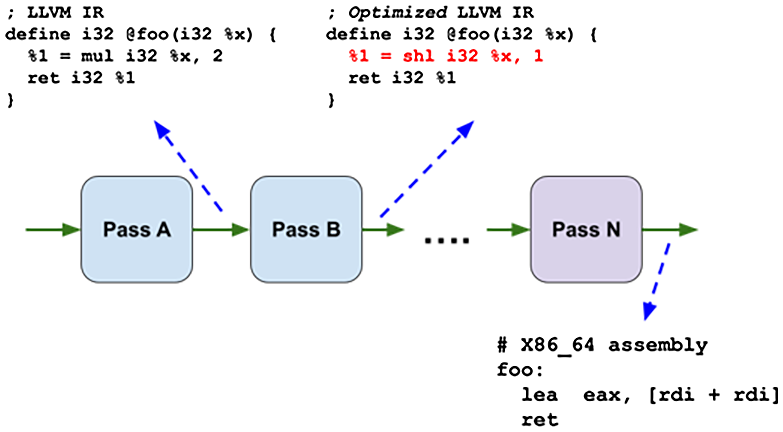
\includegraphics[width=0.9\textwidth]{content/3/chapter9/images/1.png}\\
Figure 9.1 – An example of the LLVM Pass pipeline and its intermediate results
\end{center}

In the preceding diagram, multiple Passes are arranged in a straight line. The LLVM IR for the foo function is processed by one Pass after another. Pass B, for instance, performs code optimization on foo and replaces an arithmetic multiplication (mul) by 2 with left shifting (shl) by 1, which is considered easier than multiplication in most hardware architectures. In addition, this figure also illustrates that the code generation steps are modeled as Passes. Code generation in LLVM transforms LLVM IR, which is target independent, into assembly code for certain hardware architecture (for example, x86\_64 in Figure 9.1). Each detailed procedure, such as the register allocation, instruction selection, or instruction scheduling, is encapsulated into a single Pass and is executed in a certain order.

\begin{tcolorbox}[colback=blue!5!white,colframe=blue!75!black, fonttitle=\bfseries,title=Code generation Passes]	
\hspace*{0.7cm}Passes for code generation have a different API than normal LLVM IR Passes. Additionally, during the code generation phase, LLVM IR is actually converted into another kind of IR, called Machine IR (MIR). However, in this chapter, we will only be covering LLVM IR and its Passes.
\end{tcolorbox}

This Pass pipeline is conceptually managed by an infrastructure called PassManager. PassManager owns the plan – their execution order, for example – to run these Passes. Conventionally, we actually use the terms Pass pipeline and PassManager interchangeably since they have nearly identical missions. In the Learning instrumentations in the new PassManager section, we will go into more detail about the pipeline itself and discuss how to customize the execution order of these enclosing Passes.

Code transformations in modern compilers can be complex. Because of this, multiple transformation Passes might need the same set of program information, which is called analysis in LLVM, in order to do their work. Furthermore, to achieve maximum efficiency, LLVM also caches this analysis data so that it can be reused if possible. However, since a transformation Pass might change the IR, some cached analysis data, which was previously collected, might be outdated after running that Pass. To solve these challenges, in addition to PassManager, LLVM has also created AnalysisManager to manage everything related to program analysis. We will go deeper into AnalysisManager in the Working with the new AnalysisManager section.

As mentioned in the introduction of this chapter, LLVM has gone through a series of overhauls on its Pass and PassManager (and AnalysisManager) infrastructure. The new infrastructure runs faster and generates results with better quality. Nevertheless, the new Pass differs in many places from the old one; we will briefly explain these differences along the way. However, aside from that, we will only be discussing the new Pass infrastructure, by default, for the rest of the chapter.

In this section, we will show you how to develop a simple Pass for the new PassManager. As usual, we will begin with a description of the sample project we are about to use. Then, we will show you the steps to create a Pass that can be dynamically loaded from a plugin into the Pass pipeline, which was mentioned earlier, using the opt utility.


\subsubsubsection{9.2.1\hspace{0.2cm}Project overview}

In this section, the sample project we are using is called StrictOpt. It is a Pass and Pass plugin that adds a noalias attribute to every function parameter that has a pointer type. Effectively, it adds a restrict keyword to the function parameters in C code. First, let's explain what the restrict keyword does.

\begin{tcolorbox}[colback=blue!5!white,colframe=blue!75!black, fonttitle=\bfseries,title=The restrict keyword in C and C++]	
\hspace*{0.7cm}The restrict keyword was introduced in C99. However, it doesn't have a counterpart in C++. Nevertheless, mainstream compilers such as Clang, GCC, and MSVS all support the same functionality in C++. For example, in Clang and GCC, you can use \_\_restrict\_\_ or \_\_restrict in C++ code and it has the same effect as restrict in C.
\end{tcolorbox}

The restrict keyword can also be used alongside pointer type variables in C. In the most common cases, it is used with pointer type function parameters. The following is an example:

\begin{lstlisting}[style=styleCXX]
int foo(int* restrict x, int* restrict y) {
	*x = *y + 1;
	return *y;
}
\end{lstlisting}

Essentially, this additional attribute tells the compiler that argument x will never point to the same memory region as argument y. In other words, programmers can use this keyword to persuade the compilers that they will never call the foo function, as follows:

\begin{lstlisting}[style=styleCXX]
…
// Programmers will NEVER write the following code
int main() {
	int V = 1;
	return foo(&V, &V);
}
\end{lstlisting}

The rationale behind this is that if the compiler knows that two pointers – in this case, the two pointer arguments – will never point to the same memory region, it can do more aggressive optimizations. To give you a more concrete understanding of this, if you compare the assembly code of the foo function with and without the restrict keyword, the latter version takes five instructions to execute (on x86\_64):

\begin{lstlisting}[style=stylePython]
foo:
	mov eax, dword ptr [rsi]
	add eax, 1
	mov dword ptr [rdi], eax
	mov eax, dword ptr [rsi]
	ret
\end{lstlisting}

The version with the restrict keyword added only takes four instructions:

\begin{lstlisting}[style=stylePython]
foo:
	mov eax, dword ptr [rsi]
	lea ecx, [rax + 1]
	mov dword ptr [rdi], ecx
	ret
\end{lstlisting}

Although the difference here seems subtle, in the version without restrict, the compiler needs to insert an extra memory load to assure that the last argument *y (in the original C code) always reads the latest value. This extra cost might gradually accumulate in a more complex code base and, eventually, create a performance bottleneck.

Now, you have learned how restrict works and its importance for ensuring good
performance. In LLVM IR, there is also a corresponding directive to model the restrict keyword: the noalias attribute. This attribute is attached to the  pointer function parameters if hints such as restrict have been given by programmers in  the original source code. For example, the foo function (with the restrict keywords) can be translated into the following LLVM IR:

\begin{lstlisting}[style=stylePython]
define i32 @foo(i32* noalias %0, i32* noalias %1) {
	%3 = load i32, i32* %1
	%4 = add i32 %3, 1
	store i32 %4, i32* %0
	ret i32 %3
}
\end{lstlisting}

Furthermore, we can also generate the LLVM IR code of the foo function without restrict in C code, as follows:

\begin{lstlisting}[style=stylePython]
define i32 @foo(i32* %0, i32* %1) {
	%3 = load i32, i32* %1
	%4 = add i32 %3, 1
	store i32 %4, i32* %0
	%5 = load i32, i32* %1
	ret i32 %5
}
\end{lstlisting}

Here, you will find that there is an extra memory load (as shown in the highlighted instruction of the preceding snippet), which is similar to what happened to the assembly examples from earlier. That is, LLVM is unable to perform more aggressive optimization to remove that memory load since it's not sure whether those pointers overlap each other.

In this section, we are going to write a Pass to add a noalias attribute to every pointer argument of a function. The Pass will be built as a plugin, and once it's loaded into opt, users can use the --passes argument to explicitly trigger StrictOpt, as follows:

\begin{tcblisting}{commandshell={}}
$ opt --load-pass-plugin=StrictOpt.so \
      --passes="function(strict-opt)" \
      -S -o – test.ll
\end{tcblisting}

Alternatively, we can make StrictOpt run before other optimizations if the optimization level is greater or equal to -O3. The following is an example:

\begin{tcblisting}{commandshell={}}
$ opt -O3 --enable-new-pm \
      --load-pass-plugin=StrictOpt.so \
      -S -o – test.ll
\end{tcblisting}

We will show you how to switch between these two modes shortly.

\begin{tcolorbox}[colback=blue!5!white,colframe=blue!75!black, fonttitle=\bfseries,title=A demo-only Pass]	
\hspace*{0.7cm}Note that StrictOpt is merely a demo-only Pass, and adding noalias to every pointer function argument is absolutely not the thing you should do in real-world use cases. This is because it might break the correctness of the target program.
\end{tcolorbox}

In the next section, we will show you detailed steps of how to create this Pass.

\subsubsubsection{9.2.2\hspace{0.2cm}Writing the StrictOpt Pass}

The following instructions will take you through the process of developing the core Pass logic before covering how to register StrictOpt into the Pass pipeline dynamically:

\begin{enumerate}
\item We only have two source files this time: StrictOpt.h and StrictOpt.cpp. In the former file, we place the skeleton of the StrictOpt Pass:

\begin{lstlisting}[style=styleCXX]
#include "llvm/IR/PassManager.h"
struct StrictOpt : public PassInfoMixin<StrictOpt> {
	PreservedAnalyses run(Function &F,
	  FunctionAnalysisManager &FAM);
};
\end{lstlisting}

The Pass we are writing here is a function Pass; namely, it runs on the Function IR unit. The run method is the primary entry point for this Pass, which we are going to fill in later. It takes two arguments: a Function class that we will work on and a FunctionAnalysisManager class that can give you analysis data. It returns a PreservedAnalyses instance, which tells PassManager (and AnalysisManager) what analysis data was invalidated by this Pass.

If you have prior experience in writing LLVM Pass for the legacy PassManager, you might find several differences between the legacy Pass and the new Pass:

\begin{enumerate}[label=\alph*)]
\item  The Pass class no longer derives from one of the FunctionPass, ModulePass, or LoopPass. Instead, the Passes running on different IR units are all deriving from PassInfoMixin<YOUR\_PASS>. In fact, deriving from PassInfoMixin is not even a requirement for a functional Pass anymore – we will leave this as an exercise for you.

\item  Instead of overriding methods, such as runOnFunction or runOnModule, you will define a normal class member method, run (be aware that run does not have an override keyword that follows), which operates on the desired IR unit.

\end{enumerate}

Overall, the new Pass has a cleaner interface compared to the legacy one. This difference also allows the new PassManager to have less overhead runtime.

\item To implement the skeleton from the previous step, we are heading to StrictOpt.cpp. In this file, first, we create the following method definition:

\begin{lstlisting}[style=styleCXX]
#include "StrictOpt.h"
using namespace llvm;
PreservedAnalyses StrictOpt::run(Function &F,
                                 FunctionAnalysisManager &FAM) {
	return PreservedAnalyses::all(); // Just a placeholder
}
\end{lstlisting}

The returned PreservedAnalyses::all() instance is just a placeholder that will be removed later.

\item Now, we are finally creating the code to add a noalias attribute to the pointer function arguments. The logic is simple: for each Argument instance in a Function class, attach noalias if it fulfills the criteria:

\begin{lstlisting}[style=styleCXX]
// Inside StrictOpt::run…
bool Modified = false;
for (auto &Arg : F.args()) {
	if (Arg.getType()->isPointerTy() &&
	!Arg.hasAttribute(Attribute::NoAlias)) {
		Arg.addAttr(Attribute::NoAlias);
		Modified |= true;
	}
}
\end{lstlisting}

The args() method of the Function class will return a range of Argument instances representing all of the formal parameters. We check each of their types to make sure there isn't an existing noalias attribute (which is represented by the Attribute::NoAlias enum). If everything looks good, we use addAttr to attach noalias.

Here, the Modified flag here records whether any of the arguments were modified in this function. We will use this flag shortly.

\item Certain analysis data might become outdated after a transformation Pass since the latter might change the program's IR. Therefore, when writing a Pass, we need to return a PreservedAnalyses instance to show which analysis was affected and should be subject to recalculation. While there are many analyses available in LLVM, we don't need to enumerate each of them. Instead, there are some handy utility functions to create PreservedAnalyses instances, representing all analyses or none of the analyses, such that we only need to subtract or add (un) affected analysis from it. Here is what we do in StrictOpt:

\begin{lstlisting}[style=styleCXX]
#include "llvm/Analysis/AliasAnalysis.h"
…
// Inside StrictOpt::run…
auto PA = PreservedAnalyses::all();
if (Modified)
	PA.abandon<AAManager>();
return PA;
\end{lstlisting}

Here, we first create a PreservedAnalyses instance, PA, which represents all analyses. Then, if the Function class we are working on here has been modified, we discard the AAManager analysis via the abandon method. AAManager represents the alias analysis in LLVM.

Without going into the details of this, the alias analysis asks whether two pointers point to the same memory region, or whether the memory regions they are pointing to overlap with each other. The noalias attribute we are discussing here has strong relations with this analysis since they're working on a nearly identical problem. Therefore, if any new noalias attribute was generated, all the cached alias analysis data would be outdated. This is why we invalidate it using abandon.

Note that you can always return a PreservedAnalyses::none() instance, which tells AnalysisManager to mark every analysis as outdated if you are not sure what analyses have been affected. This comes at a cost, of course, since AnalysisManager then needs to spend extra effort to recalculate the analyses that might contain expensive computations.

\item The core logic of StrictOpt is essentially finished. Now, we are going to show you how to dynamically register the Pass into the pipeline. In StrictOpt.cpp, we create a special global function, called llvmGetPassPluginInfo, with an outline like this:

\begin{lstlisting}[style=styleCXX]
extern "C" ::llvm::PassPluginLibraryInfo LLVM_ATTRIBUTE_
WEAK
llvmGetPassPluginInfo() {
	return {
		LLVM_PLUGIN_API_VERSION, "StrictOpt", "v0.1",
		[](PassBuilder &PB) {…}
	};
}
\end{lstlisting}
 
This function returns a PassPluginLibraryInfo instance, which contains various pieces of information such as the plugin API version (LLVM\_PLUGIN\_API\_VERSION) and the Pass name (StrictOpt). One of its most important fields is a lambda function that takes a single PassBuilder\& argument. In that particular function, we are going to insert our StrictOpt into a proper position within the Pass pipeline.

PassBuilder, as its name suggests, is an entity LLVM that is used to build the Pass pipeline. In addition to its primary job, which involves configuring the pipeline according to the optimization level, it also allows developers to insert Passes into some of the places in the pipeline. Furthermore, to increase its flexibility, PassBuilder allows you to specify a textual description of the pipeline you want to run by using the --passes argument on opt, as we have seen previously. For instance, the following command will run InstCombine, PromoteMemToReg, and SROA (SROA: Scalar Replacement of Aggregates) in sequential order:

\begin{tcblisting}{commandshell={}}
$ opt --passes="instcombine,mem2reg,sroa" test.ll -S -o –
\end{tcblisting}

What we are going to do in this step is ensure that after the plugin has been loaded, opt will run our Pass if strict-opt appears in the --passes argument, as follows:

\begin{tcblisting}{commandshell={}}
$ opt --passes="strict-opt" test.ll -S -o –
\end{tcblisting}

To do this, we leverage the registerPipelineParsingCallback method in PassBuilder:

\begin{lstlisting}[style=styleCXX]
…
[](PassBuilder &PB) {
	using PipelineElement = typename
	PassBuilder::PipelineElement;
	PB.registerPipelineParsingCallback(
	[](StringRef Name,
	FunctionPassManager &FPM, ArrayRef<PipelineElement>){
		if (Name == "strict-opt") {
			FPM.addPass(StrictOpt());
			return true;
		}
		return false;
	});
}
\end{lstlisting}

The registerPipelineParsingCallback method takes another lambda callback as the argument. This callback is invoked whenever PassBuilder encounters an unrecognized Pass name while parsing the textual pipeline representation. Therefore, in our implementation, we simply insert our StrictOpt pass into the pipeline via FunctionPassManager::addPass when the unrecognized Pass name, that is, the Name parameter, is strict-opt.

\item Alternatively, we also want to trigger our StrictOpt at the beginning of the Pass pipeline without using the textual pipeline description, as we described in the Project overview section. This means that the Pass will be run before other Passes after it is loaded into opt using the following command:

\begin{tcblisting}{commandshell={}}
$ opt -O2 --enable-new-pm \
      --load-pass-plugin=StrictOpt.so test.ll -S -o –
\end{tcblisting}

(The --enable-new-pm flag in the preceding command forced opt to use the new PassManager since it's still using the legacy one by default. We haven't used this flag before because --passes implicitly enables the new PassManager under the hood.)

To do this, instead of using PassBuilder::registerPipelineParsingCallback to register a custom (pipeline) parser callback, we are going to use  registerPipelineStartEPCallback to handle this. Here is the alternative version of the code snippet from the previous step:

\begin{lstlisting}[style=styleCXX]
…
[](PassBuilder &PB) {
	using OptimizationLevel
	= typename PassBuilder::OptimizationLevel;
	PB.registerPipelineStartEPCallback(
	[](ModulePassManager &MPM, OptimizationLevel OL) {
		if (OL.getSpeedupLevel() >= 2) {
			MPM.addPass(
			createModuleToFunctionPassAdaptor(StrictOpt()));
		}
	});
}
\end{lstlisting}

\begin{itemize}
\item The registerPipelineStartEPCallback method we are using here registers
a callback that can customize certain places in the Pass pipeline, called extension points (EPs). The EP we are going to customize here is one of the earliest points in the pipeline.

\item In comparison to the lambda callback we saw in registerPipelineParsingCallback, the lambda callback for registerPipelineStartEPCallback only provides ModulePassManager, rather than FunctionPassManager, to insert our StrictOpt Pass, which is a function Pass. We are using ModuleToFunctionPassAdapter to overcome this issue.

ModuleToFunctionPassAdapter is a module Pass that can run a given function Pass over a module's enclosing functions. It is suitable for running a function Pass in contexts where only ModulePassManager is available, such as in this scenario. The createModuleToFunctionPassAdaptor function highlighted in the preceding code is used to create a new  ModuleToFunctionPassAdapter instance from a specific function Pass.

\item Finally, in this version, we are only enabling StrictOpt when the optimization level is greater or equal to -O2. Therefore, we leverage the OptimizationLevel argument passing into the lambda callback to determine whether we want to insert StrictOpt into the pipeline or not.

With these Pass registration steps, we have also learned how to trigger our StrictOpt without explicitly specifying the textual Pass pipeline.
\end{itemize}

To summarize, in this section, we learned the essentials of the LLVM Pass and Pass pipeline. Through the StrictOpt project, we have learned how to develop a Pass – which is also encapsulated as a plugin – for the new PassManager and how to dynamically register it against the Pass pipeline in opt in two different ways: first, by triggering the Pass explicitly via a textual description, and second, by running it at a certain time point (EP) in the pipeline. We also learned how to invalidate analyses depending on the changes made in the Pass. These skills can help you develop high-quality and modern LLVM Passes to process IR in a composable fashion with maximum flexibility. In the next section, we will dive into the program analysis infrastructure of LLVM. This greatly improves the capability of normal LLVM transformation Passes.

\end{enumerate}






























